%\documentclass{book}\usepackage{sjtfonts}\usepackage{includegraphics}\usepackage{alltt}\usepackage{latexsym}
%\usepackage{array}
%\begin{document}\input{defs0}%		miradefs.tex 		    June 1994

% opening and closing a quoted Miranda section

\newcommand{\mira}{\noindent\hrulefill\nopagebreak\so}
\newcommand{\arim}{\nopagebreak\st\hrulefill\\}

% backslash in the Miranda environment
% Only feasible approach is to use \verb+\+
% in line!

%\newcommand{\bs}{$\mi\backslash\!\!$}
%\newcommand{\lbs}{\mbox{\verb+\+}}

% ignoring part of the input

\newcommand{\ignore}[1]{}

% a blank line in a Miranda section

\newcommand{\bl}{\mbox{\ }}

% Signalling a diffculty.

\definecolor{light-gray}{gray}{0.95}

\newcommand{\beware}[2]
 {\medskip\noindent\colorbox{light-gray}{\parbox{\textwidth}
 {\mbox{\large\textbf{#1}} \medskip\noindent\\ #2}\medskip\noindent}}

% Subscripting in Miranda text
\newcommand{\subscr}[2]{\mbox{${\mbox{\texttt{#1}}}_{\mbox{\texttt{#2}}}$}}

%\newcommand{\subscr}[2]{\mbox{${\mbox{\mi #1}}_{\mbox{\smtt #2}}$}}
\newcommand{\aone}{\subscr{a}{1}}
\newcommand{\atwo}{\subscr{a}{2}}
\newcommand{\ak}{\subscr{a}{k}}

\newcommand{\aoneone}{\subscr{a}{1,1}}

\newcommand{\eone}{\subscr{e}{1}}
\newcommand{\etwo}{\subscr{e}{2}}
\newcommand{\ei}{\subscr{e}{i}}
\newcommand{\er}{\subscr{e}{r}}

\newcommand{\fone}{\subscr{f}{1}}
\newcommand{\fl}{\subscr{f}{l}}

\newcommand{\gone}{\subscr{g}{1}}
\newcommand{\gtwo}{\subscr{g}{2}}
\newcommand{\gi}{\subscr{g}{i}}
\newcommand{\gr}{\subscr{g}{r}}

\newcommand{\hone}{\subscr{h}{1}}
\newcommand{\hl}{\subscr{h}{l}}

\newcommand{\pone}{\subscr{p}{1}}
\newcommand{\ptwo}{\subscr{p}{2}}
\newcommand{\pk}{\subscr{p}{k}}

\newcommand{\qone}{\subscr{q}{1}}
\newcommand{\qtwo}{\subscr{q}{2}}
\newcommand{\qk}{\subscr{q}{k}}

\newcommand{\rone}{\subscr{r}{1}}
\newcommand{\rtwo}{\subscr{r}{2}}

\newcommand{\tone}{\subscr{t}{1}}
\newcommand{\ttwo}{\subscr{t}{2}}
\newcommand{\tn}{\subscr{t}{n}}

\newcommand{\vone}{\subscr{v}{1}}
\newcommand{\vtwo}{\subscr{v}{2}}
\newcommand{\vn}{\subscr{v}{n}}

% for regular expressions

\newcommand{\stone}{\subscr{st}{1}}
\newcommand{\sttwo}{\subscr{st}{2}}
\newcommand{\stn}{\subscr{st}{n}}
\newcommand{\rthree}{\subscr{r}{3}}

\newcommand{\eps}{$\varepsilon$}
\newcommand{\trans}[1]{\stackrel{\mbox{\tt #1}}{\longrightarrow}}



% superscript in Miranda text

\newcommand{\superscr}[2]{\mbox{${\mbox{\mi #1}}^{\mbox{\smtt #2}}$}}

% Not equals in Miranda text

\newcommand{\noteq}{\makebox[0pt][l]{=}/}
\newcommand{\overslash}{\makebox[0pt][l]{/}}

% Definitions in complexity chapter

\newfont{\oldSym}{cmsy10}
\newcommand{\Th}{\boldmath$\oldSym\Theta$}
\newcommand{\pow}[1]{\^{}#1}
\newcommand{\leqq}{$\leq$}
\newcommand{\geqq}{$\geq$}
\newcommand{\lll}{$\ll$}
\newcommand{\eqq}{$\equiv$}
\newcommand{\ltwo}{\subscr{log}{2}}

% Indexing

\newcommand{\minx}[1]{\index{#1@{\ttfamily{}#1}}}
\setcounter{chapter}{7}\setcounter{page}{127}

\chapter{Reasoning about programs}
\chapstart
\label{reasoningProgs}
\index{reasoning|see{proof}}
\index{proof|(}


We gave an introduction to proof in Section \ref{proof}, where we said
that a \emph{proof} is an argument that a particular proposition
holds. Often
a proposition will be \emph{general} in saying that something holds
\emph{for all} 
things of a certain sort. In mathematics we might give a proof of Pythagoras'
theorem, which states that there is a relationship {\tt a$^{\tt 2}$=b$^{\tt
2}$+c$^{\tt 2}$} between the sides of all right-angled triangles. 

In programming we can prove that programs have
a particular property \emph{for all} input values. Having a proof
means that we can be certain that the program will behave as we require
whatever the conditions. Compare this with program testing: a test
assures us that a program behaves as it should on a particular collection of input
values; it can only be an act of faith to infer from this that the program behaves as
expected on every possible input, and no mathematician would accept a proposition
as valid simply because it holds for a limited set of test data. 


Property-based testing -- as given by QuickCheck -- provides much better coverage, but it is still possible that the places where an error occurs could be missed by randomly generating data; proof avoids this, and gives an error `nowhere to hide': Figure \ref{TPP} on page \pageref{TPP} illustrates this. Even when we are sure that using QuickCheck shows that a particular property holds, a proof can tell us \emph{why} that property holds, not just that it is true.

Central to applying proof within functional programming is
the insight that we can read function definitions as \emph{logical
descriptions} of what they do; we discuss this in depth at the
start of the chapter. After looking again at the relationship of reasoning, testing and property-based testing, we look at some background topics in programming and logic,
before introducing the central idea of proof by induction over finite
lists.

Proofs by induction follow a pattern, and we illustrate this by giving a
sequence of examples. We also supply advice on how to go about finding
induction proofs. We also look at the QuickCheck properties that correspond to the propositions we prove, and indeed check them using QuickCheck.  The chapter concludes with a more challenging example
of proof, which you can omits on a first reading.

\section{Understanding definitions}

Suppose that we ask ourselves the seemingly obvious question: `how
do we understand what a function does?' There are various ways
of answering this. 
\begin{itemize}
\item We can evaluate what the function does on particular inputs, using an
implementation like GHCi.
\item We can do the same thing by hand, performing a line-by-line
calculation. This has the advantage of letting us see how the program
gets to its result, but the disadvantage of being slow and impractical
for all but the smallest of programs.
\item We can try to argue about how the program behaves in general. 
\end{itemize}
The third answer, in which we reason about the behaviour of our
programs, is the subject of this chapter, which builds on the
introduction of Section \ref{proof}.

Consider a simple functional program like
\begin{alltt}\minx{length}
length []     = 0\hfill(length.1)
length (x:xs) = 1 + length xs\hfill(length.2)
\end{alltt}
Using the definition we can calculate the length of any particular list
like [2,3,1]
\begin{alltt}
length [2,3,1]
\step 1 + length [3,1]\hfill\textrm{by }(length.2)
\step 1 + (1 + length [1])\hfill\textrm{by }(length.2)
\step 1 + (1 + (1 + length []))\hfill\textrm{by }(length.2)
\step 1 + (1 + (1 + 0))\hfill\textrm{by }(length.1)
\step 3
\end{alltt}
We can also read \texttt{(length.1)} and \texttt{(length.2)} as
\textbf{descriptions} of how \texttt{length} behaves in general.
\begin{itemize}
\item \texttt{(length.1)} says what \texttt{length []} is;
\item \texttt{(length.2)} says that \textbf{whatever values} of
\texttt{x} and \texttt{xs} we choose, \texttt{length (x:xs)} will be
equal to \texttt{1 + length xs}.
\end{itemize}
In the second case we have a \textbf{general property} of
\texttt{length}: it states something about
how length behaves on all non-empty lists.
On the basis of these equations we can conclude that 
\begin{alltt}
length [x] = 1\hfill(length.3)
\end{alltt}
How do we do that? We know that \texttt{(length.2)} holds for \textbf{all} 
values of \texttt{x} and \texttt{xs}, and so it will hold in particular
when \texttt{xs} is replaced by \texttt{[]}, so
\begin{alltt}
length [x] 
  = length (x:[])\hfill\textrm{by defn of \texttt[x]}
  = 1 + length []\hfill\textrm{by }(length.2)
  = 1 + 0 \hfill\textrm{by }(length.1)
  = 1
\end{alltt}
The lesson of this discussion is that we can read a function definition in
(at least) two different ways.
\begin{itemize}
\item We can take the definition as describing how to compute particular
results, such as \texttt{length [2,3,1]}.
\item We can also take the definition as a \textbf{general description}
of the behaviour of the function in question.
\index{function definition!as description}
\end{itemize}
From this general description we are able to deduce other facts, some
like
\texttt{(length.3)} being
utterly straightforward, and others like
\begin{alltt}
length (xs ++ ys) = length xs + length ys\hfill(length.4) 
\end{alltt}
expressing more complicated interactions between two or more
functions. We will prove \texttt{(length.4)} in Section \ref{furtherIndPrfs}.

Another way of looking at the proof of \texttt{(length.3)} above is that
we are doing \textbf{symbolic evaluation}; rather than evaluating
\index{symbolic evaluation}\index{evaluation!symbolic}
\texttt{length} at a particular value like \texttt{[2]} we have replaced
the number \texttt{2}
with a variable \texttt{x}, but used the evaluation rules in exactly
the way that we used them earlier. We will find that symbolic
evaluation forms an important part of our proofs, but we will need to
use another principle -- induction -- to do most proofs for recursive
functions.

To conclude this introduction, we have seen that functional programs
`describe themselves' in a direct way. If you are familiar with an
imperative language like Pascal, C or Java, think how you might convince
yourself of the analogues of \texttt{(length.3)}
or \texttt{(length.4)} for programs written in that language. 
It's very difficult to see how you might state
these properties, and even more difficult to work out how to prove them valid.

\section{Testing and proof}
\index{proof!and testing}
\index{proof!and QuickCheck}
\index{testing!and proof}
\index{QuickCheck!and proof}

When we introduced program testing in Section \ref{testing} we looked at the example
\begin{alltt}\minx{mysteryMax}
mysteryMax :: Integer -> Integer -> Integer -> Integer
mysteryMax x y z
  | x > y \&\& x > z      = x
  | y > x \&\& y > z      = y
  | otherwise           = z
\end{alltt} 
which was an attempted solution to the problem of finding the maximum of three integers.


If I asked you to give me five sets of test data for the function, and for you to test the function at those points, I would guess that you would conclude that the implementation works: try it!

We can write a \textbf{property}\index{property} that expresses that the function does as it should, like this:
\begin{alltt}\minx{prop\_mystery}
prop_mystery :: Integer -> Integer -> Integer -> Bool

prop_mystery x y z =
    mysteryMax x y z == (x `max` y) `max` z
\end{alltt} 
Let's see what happens when we check this property using QuickCheck:
\begin{alltt}
\textsl{*Chapter8>} quickCheck prop_mystery
\textsl{*** Failed! Falsifiable (after 91 tests and 2 shrinks):     
75
75
0
*Chapter8 Test.QuickCheck>} quickCheck prop_mystery
\textsl{*** Failed! Falsifiable (after 4 tests and 1 shrink):     
3
3
0
*Chapter8>} quickCheck prop_mystery
\textsl{+++ OK, passed 100 tests.}
\end{alltt}
The first time we check it, it takes 91 tests to find the error; in the second case we find it much more quickly, but in the third we don't catch it at all!

Now let's try to \textbf{prove} that the function behaves as it should. 
We need to look at various \emph{cases} of
the ordering of the values. If we first look at the cases
\begin{alltt}
x > y \&\& x > z
y > x \&\& y > z
z > x \&\& z > y
\end{alltt} 
then in each of these \texttt{mysteryMax} will produce the correct
solution. In the other cases, at least two of the three arguments are equal. If all three 
are equal,
\begin{alltt}
x == y \&\& y == z
\end{alltt}
the function also operates correctly. Finally, we start to look at the
cases where precisely two elements are equal. The function behaves
correctly when
\begin{alltt}
y == z \&\& z > x
\end{alltt}
but in the case of
\begin{alltt}
x == y \&\& y > z
\end{alltt}
we can see that the result will, erroneously, be \texttt{z}. 

Now, we can
see this process of attempting to prove a result as a general way of
testing the function -- it is a form of \textbf{symbolic testing} which
will consider all cases in turn, at least until an error is found. We can therefore see that reasoning can give us a powerful way
of debugging\index{debugging} programs by focusing on the reason why we cannot complete a proof of
correctness, as well as the more traditional view that a proof shows that a program 
meets the requirements put upon it.

On the other hand, as we mentioned in Section \ref{testing}, finding a proof is a
difficult enterprise, and so there are clearly roles for 
proof, property-based testing and traditional testing  in the development of reliable software. 


\section{Definedness, termination and finiteness}
\index{finiteness}

Before we say anything more about proof, we need to talk about two aspects of
programming upon which we have only touched so far. 

\subsection*{Definedness and termination}
\index{definedness}
\index{evaluation!definedness of}

Evaluating an expression
can have one of two outcomes:

\begin{titemize}
\item the evaluation can halt, or \textbf{terminate}, to give an answer; or
\index{termination}
\item the evaluation can go on forever.
\end{titemize}
If we make the definition
\begin{alltt}
fact :: Integer -> Integer
fact n
  | n==0        = 1
  | otherwise   = n * fact (n-1)
\end{alltt}
then examples of the two are given by the expressions
\begin{alltt}
fact 2                     fact (-2)
\end{alltt}
since in the latter case
\begin{alltt}
fact (-2)
\step (-2) * fact (-3)
\step (-2) * ((-3) * fact (-4))
\step ...
\end{alltt}
In the case that evaluation goes on for ever, we say that
the value of the expression is \textbf{undefined}, since no defined result is reached. In
writing proofs we often have to confine our attention to cases where a
value is \textbf{defined}, since it is only for defined values that many familiar
properties hold. One of the simplest examples is given by the expression
\begin{alltt}
0*e
\end{alltt}
which we expect to be \texttt{0} irrespective of the value of \texttt{e}.
That is certainly so if \texttt{e} has a defined
value, but if \texttt{e} is \texttt{fact (-2)}, the value of 
\begin{alltt}
0 * fact (-2)
\end{alltt}
will be undefined and {\em not\/} zero.

In many of the proofs we give, we state that results hold for all
defined values. This restriction does not cause problems in practice,
since the defined cases will be exactly those which interest
us the vast majority of the time. An undefined value {\it is\/}
of interest when a function does not give a defined value when it is
expected to -- a case of symbolic debugging.

\subsection*{Finiteness}
\index{finiteness}

We have said nothing so far about the order in which expressions are
evaluated in Haskell. In fact, Haskell evaluation is \textbf{lazy}, so
that arguments to functions are only evaluated if their values are
actually needed. This gives some Haskell programs a
distinctive flavour, which we explore in depth in Chapter \ref{lazy}.
What is important for us here is that lazy evaluation allows the
definition and use of \textbf{infinite} lists like\index{lists!infinite}
\begin{alltt}
[1,2,3, ... ]
\end{alltt}
and \textbf{partially defined}\index{lists!partially defined}
lists. In what follows we will
mainly confine our attention to \textbf{finite} lists, by which we mean
lists which have a defined, finite length and defined elements.
Examples are
\begin{alltt}
[]             [1,2,3]             [[4,5],[3,2,1],[]]
\end{alltt}
Reasoning about lazy programs is discussed explicitly
in Section \ref{lazyProof} below.

\begin{exercises}
\item
Given the definition of \texttt{fact} above, what are the results of
evaluating the following expressions?
\begin{alltt}
(4 > 2) || (fact (-1) == 17)
(4 > 2) \&\& (fact (-1) == 17)
\end{alltt}
Discuss the reasons why you think that you obtained these answers.

\item
Give a definition of a multiplication function
\begin{alltt}
mult :: Integer -> Integer -> Integer
\end{alltt}
so that \texttt{\ mult 0 (fact (-2))} evaluates to \texttt{0}.\\
What is the result of \texttt{\ mult (fact (-2)) 0} for your function?
Explain why.
\end{exercises}
\section{A little logic}

In order to appreciate how to reason about functional programs we
need not have a background in formal logic. Nevertheless, it is worth
discussing two aspects of logic before we proceed with our proofs.

\subsection*{Assumptions in proofs}

\newcommand{\poundSymbol}{\symbol{163}}

First, we look at the idea of proofs
which contain {\bf assumptions}\index{assumptions}.
Taking a particular example,
it follows from elementary arithmetic
that 
if we {\em assume\/} that petrol costs 27 pence per litre,
then we can prove that four litres will cost \pounds 1.08. 

What does this tell us? It does {\em not\/} tell us outright how much four
litres will cost; it only tells us the cost {\em if the assumption is valid}. To be
sure that
the cost will be \pounds 1.08, we need to supply some evidence that the
assumption is justified: this might be another proof --- perhaps based on
petrol costing \pounds 1.20 per gallon --- or direct evidence.

We can write what we have proved as a formula,
\[
\mbox{1 litre costs 27 pence \imp\ 4 litres cost \pounds 1.08}
\index{\imp@{\imp}}
\]
where the arrow, \imp, which is the logical symbol for
\textbf{implication},\index{implication@implication (\(\Rightarrow\))}
says that the second proposition
\textbf{follows from} the first. 

As we have seen, we prove an implication like $A\imp{}B$ by
assuming $A$ in proving $B$. If we then find a proof of $A$, then knowing the implication
will guarantee that $B$ is also valid. 

Yet another way of looking at this is to
see a proof of $A\imp{}B$ as a \emph{process} for turning a proof of $A$
into a proof of $B$.
We use this idea in proof by induction, as one of the tasks in building an
induction proof is the induction step, where we prove that one property
holds assuming another. 

\subsection*{Free variables and quantifiers}
\index{free variable}\index{variable!free}
\index{universal quantifier}\index{quantifier, universal}
\index{all@\all{}}

When we write an equation like
\begin{alltt}
square x = x*x
\end{alltt}
it is usually our intention to say that this holds \textbf{for all} (defined)
values of the free variable \texttt{x}. If we want to make this `for all' explicit we can
use a \textbf{quantifier} like this
\begin{alltt}
\all{}x (square x = x*x)
\end{alltt}
where we read the universal quantifier, `\texttt{\all{}x}', as saying
`for all \texttt{x}\ldots'.

\medskip

\noindent We now turn to induction, the main technique we use for proving
properties of programs.

\section{Induction}
\index{induction|(}

In Chapter \ref{defFunLists} we saw that a general method for defining lists was
primitive recursion, as exemplified by
\begin{alltt}
sum :: [Integer] -> Integer
sum []     = 0\hfill(sum.1)
sum (x:xs) = x + sum xs\hfill(sum.2)
\end{alltt}
Here we give a value outright at \texttt{[]}, and define the value of
\texttt{sum (x:xs)} using the value \texttt{sum xs}. Structural induction is a
proof principle which states:
\begin{definition}{{\sffamily Principle of structural induction for
lists}\index{structural induction}\index{structural induction!for
lists}\index{induction!for lists}


\medskip
\noindent
In order to prove that a logical property \texttt{P(xs)} holds for all \textbf{finite} lists
\texttt{xs} we have to do two things.
\begin{itemize}\index{induction!base case}
\item{\bf Base case.} Prove \texttt{P([])} outright.
\item{\bf Induction step.} Prove \texttt{P(x:xs)} on
\index{induction!induction step}the {\em assumption\/} that \texttt{P(xs)} holds. 

In other words 
\texttt{P(xs) \imp\ P(x:xs)} has to be proved.

The \texttt{P(xs)}
here is called the \textbf{induction hypothesis} since it is assumed in proving
\texttt{P(x:xs)}.
\index{induction!induction hypothesis}
\end{itemize}}
\end{definition}
It is interesting to see that this is just like primitive recursion,
except that instead of building the values of a function, we are
building up the parts of a proof. 
In both cases we deal with \texttt{[]}
as a basis, and then build the general thing by showing how to go from
\texttt{xs} to \texttt{(x:xs)}. In a function definition we define
\texttt{fun (x:xs)} using \texttt{fun xs}; in the proof of \texttt{P(x:xs)}
we are allowed to use \texttt{P(xs)}.

\subsection*{Justification}
\index{induction!justification of}

Just as we argued that recursion was not circular, so we can see proof
by induction building up the proof for all finite lists in stages. Suppose that we
are given proofs of
\texttt{P([])} and \texttt{P(xs) \imp\ P(x:xs)} for all \texttt{x} and \texttt{xs}
and we want to show that
\texttt{P([1,2,3])}. The list \texttt{[1,2,3]} is built up from
\texttt{[]} using cons like this,
\begin{alltt}
1:2:3:[]
\end{alltt}
and we can construct the proof of \texttt{P([1,2,3])} in a way which
mirrors this
step-by-step construction,
\begin{titemize}
\item \texttt{P([])} holds;
\item \texttt{P([]) \imp\ P([3])} holds, since it is a case of
\texttt{P(xs) \imp\ P(x:xs)};
\item Recall our
discussion of `\imp' above; if we know that both \texttt{P([]) \imp\ P([3])} and 
\texttt{P([])} hold, then 
we can infer that \texttt{P([3])} holds.
\item \texttt{P([3]) \imp\ P([2,3])} holds, and so for similar reasons
we get \texttt{P([2,3])}.
\item Finally, because \texttt{P([2,3]) \imp\ P([1,2,3])} holds,
we see that \texttt{P([1,2,3])} holds.
\end{titemize}
This explanation is for a particular finite list, but will work for any finite list: if
the list has \texttt{n} elements, then we will have \texttt{n+1} steps like the four above.
To conclude, this shows that we get \texttt{P(xs)} for every possible \textbf{finite} list 
\texttt{xs} if we know that both requirements of the induction principle hold.

\subsection*{A first example}

We have mentioned the definition of \texttt{sum}; recall also the
function to double all elements of a list
\begin{alltt}\minx{doubleAll}
doubleAll []     = []\hfill(doubleAll.1)
doubleAll (z:zs) = 2*z : doubleAll zs\hfill(doubleAll.2)
\end{alltt}
Now, how would we expect \texttt{doubleAll} and \texttt{sum} to
interact? If we \texttt{sum} a list after doubling all its elements, we
would expect to get the same result as by doubling the sum of the original
list:
\begin{alltt}\minx{sum}
sum (doubleAll xs) = 2 * sum xs\hfill(sum+dblAll)
\end{alltt}
We can make this a QuickCheck\index{QuickCheck} property, like this:
\begin{alltt}\minx{prop\_SumDoubleAll}
prop_SumDoubleAll :: [Integer] -> Bool

prop_SumDoubleAll xs =
    sum (doubleAll xs) == 2 * sum xs
\end{alltt}
which is identical except that we use the Boolean equality `\texttt{==}' rather than the mathematical equality `\texttt{=}'; the property repeatedly passes 100 tests when we QuickCheck it.


\subsubsection*{Setting up the induction}

How are we to prove this for all \texttt{xs}? According to the principle of structural induction
we get two induction goals. The first is the base case
\begin{alltt}
sum (doubleAll []) = 2 * sum []\hfill(base)
\end{alltt}
The second is the induction step, in which we have to prove
\begin{alltt}
sum (doubleAll (x:xs)) = 2 * sum (x:xs)\hfill(ind)
\end{alltt}
using the induction hypothesis 
\begin{alltt}
sum (doubleAll xs) = 2 * sum xs\hfill(hyp)
\end{alltt}
In all proofs that follow we will label the cases by \texttt{(base)}, \texttt{(ind)}
and \texttt{(hyp)}.
\index{base@\texttt{(base)}}
\index{ind@\texttt{(ind)}}
\index{hyp@\texttt{(hyp)}}

\subsubsection*{The base case}

We are required to prove \texttt{(base)}: how do we start?
The only resources we have are the equations \texttt{(sum.1)}, \texttt{(sum.2)},
\texttt{(doubleAll.1)} and \texttt{(doubleAll.2)}, so we have to
concentrate on using these. As we are trying to prove an equation, we
can think of simplifying the two sides separately, so working with the
left-hand side first,
\begin{alltt}
sum (doubleAll [])
  = sum [] \hfill \textrm{by }(doubleAll.1)
  = 0 \hfill \textrm{by }(sum.1)
\end{alltt}
Looking at the right-hand side, we have
\begin{alltt}
2 * sum []
  = 2 * 0  \hfill \textrm{by }(sum.1)
  = 0 \hfill \textrm{by }*
\end{alltt}
This shows that the two sides are the same, and so completes the proof of the base
case.

\subsubsection*{The induction step}

Here we are required to prove \texttt{(ind)}. As in the base
case we have the defining equations of \texttt{doubleAll}
and \texttt{sum}, but we also can -- and usually {\em should\/} -- use
the induction hypothesis \texttt{(hyp)}.

We work as we did in the base case, simplifying each side as much as we
can using the defining equations. First the left-hand side,
\begin{alltt}
sum (doubleAll (x:xs))
  = sum (2*x : doubleAll xs)\hfill \textrm{by }(doubleAll.2)
  = 2*x + sum (doubleAll xs)\hfill \textrm{by }(sum.2)
\end{alltt}
and then the right
\begin{alltt}
2 * sum (x:xs)
  = 2 * (x + sum xs)\hfill \textrm{by }(sum.2)
  = 2*x + 2 * sum xs\hfill \textrm{by arith.}
\end{alltt}
Now, we have simplified each side using the defining equations. The last
step equating the two is given by the induction hypothesis
\texttt{(hyp)}, which can be used to carry on the simplification of the left-hand side, giving 
\begin{alltt}
sum (doubleAll (x:xs))
  = sum (2*x : doubleAll xs)
  = 2*x + sum (doubleAll xs)
  = 2*x + 2 * sum xs\hfill \textrm{by }(hyp)
\end{alltt}
and so this final step makes the left- and right-hand sides equal, on the
assumption that the induction hypothesis holds. This completes the
induction step, and therefore the proof itself.\blackbox\index{\blackbox@{\rule{8pt}{8pt}}}

\medskip
\noindent
We use the box, \rule{8pt}{8pt}\ , to signify the end of a proof.

\subsection*{Finding induction proofs}
\index{induction!finding proofs}

Looking at the previous example, we can glean a number of pieces of
advice about how to find proofs of properties of recursively defined
functions.
\begin{itemize}
\item As a first step, it is a good idea to \textbf{state the goal as a QuickCheck property}.\index{QuickCheck} Once we have that we can check that it should be possible to prove it: if we find a counterexample then we'd better try to reformulate the goal, and not waste our time trying to prove something that doesn't hold!
\item State clearly the goal of the induction and the two sub-goals of the
induction proof: \texttt{(base)} and \texttt{(hyp) \imp\ (ind)}.
\item If any confusion is possible, change the names of the variables
in the relevant definitions so that they are different from the
variable(s) over which you are doing the induction.
\item The only resources available are the definitions of the functions
involved and the general rules of arithmetic. 
Use these to simplify the sub-goals. If the sub-goal is an
equation, then simplify each side separately.
\item In the case of the induction step, \texttt{(ind)}, you should expect to use the
induction hypothesis \texttt{(hyp)} in your proof; if you do not, then it is most
likely that your proof is incorrect.
\item Label each step of your proof with its justification: this is
usually one of the defining equations of a function.
\end{itemize}
In the next section we look at a series of examples.

\section{Further examples of proofs by induction}
\label{furtherIndPrfs}
In this section we present two more examples of proof by structural induction
over finite lists.
\begin{example}
\subsubexample*{1. \texttt{length} and \texttt{++}}\minx{length}\minx{++}
We begin by looking at the example \texttt{(length.4)} introduced
at the start of the chapter.
\begin{alltt}
length (xs ++ ys) = length xs + length ys\hfill(length.4) 
\end{alltt}
The Quick Check property expressing this is 
\begin{alltt}\minx{prop\_lengthPlusPlus}
prop_lengthPlusPlus :: [a] -> [a] -> Bool

prop_lengthPlusPlus xs ys =
    length (xs ++ ys) == length xs + length ys
\end{alltt}
and this is verified when the property is checked.
Recall the definitions of \texttt{length} and \texttt{++}
\begin{alltt}
length []     = 0\hfill(length.1)
length (z:zs) = 1 + length zs\hfill(length.2)
 
[]     ++ zs = zs\hfill(++.1)
(w:ws) ++ zs = w:(ws++zs)\hfill(++.2)
\end{alltt}
where we have chosen new names for the variables so as not to conflict
with the variables in the goal.

\index{induction!choice of induction variable}
There is some question about how to proceed with the proof, since
\texttt{(length.4)} involves two variables, \texttt{xs} and \texttt{ys}.
We can be guided by the definitions, where we see that the definition
of \texttt{++} is made by recursion over the {\em first\/} variable. We
therefore make the goal a proof of \texttt{(length.4)} for all finite
\texttt{xs} and \texttt{ys} by induction over \texttt{xs}; the proof
works for all \texttt{ys} as \texttt{ys} is a variable, which stands for
an \textbf{arbitrary} list, just like the variable \texttt{x} in the earlier proof of
\texttt{(length.3)} stood for an arbitrary list element.
\subparagraph*{Statement} We can now write down the two goals of the induction
proof. The base case requires that we prove
\begin{alltt}
length ([] ++ ys) = length [] + length ys\hfill(base) 
\end{alltt}
and in the induction step we have to prove
\begin{alltt}
length ((x:xs) ++ ys) = length (x:xs) + length ys\hfill(ind) 
\end{alltt}
from the inductive assumption
\begin{alltt}
length (xs ++ ys) = length xs + length ys\hfill(hyp) 
\end{alltt}

\subparagraph*{Base} We look separately at the two sides of \texttt{(base)}, left-hand
side first,
\begin{alltt}
length ([] ++ ys)
  = length ys\hfill \textrm{by }(++.1)

length [] + length ys
  = 0 + length ys\hfill \textrm{by }(length.1)
  = length ys
\end{alltt}
which shows their equality.

\subparagraph*{Induction} First we look at the left-hand side of \texttt{(ind)}
\begin{alltt}
length ((x:xs) ++ ys)
  = length (x:(xs ++ ys))\hfill \textrm{by }(++.2)
  = 1 + length (xs ++ ys)\hfill \textrm{by }(length.2)
\end{alltt}
We cannot simplify this further with the defining equations, but we can
use \texttt{(hyp)} to give us
\begin{alltt}
  = 1 + length xs + length ys\hfill \textrm{by }(hyp)
\end{alltt}
Now, looking at the right-hand side of \texttt{(ind)} we get
\begin{alltt}
length (x:xs) + length ys
  = 1 + length xs + length ys\hfill \textrm{by }(length.2)
\end{alltt}
and this shows that \texttt{(ind)} follows from \texttt{(hyp)},
completing the second half of the proof and so the proof itself.\blackbox

\begin{figure}[t]
\begin{center}
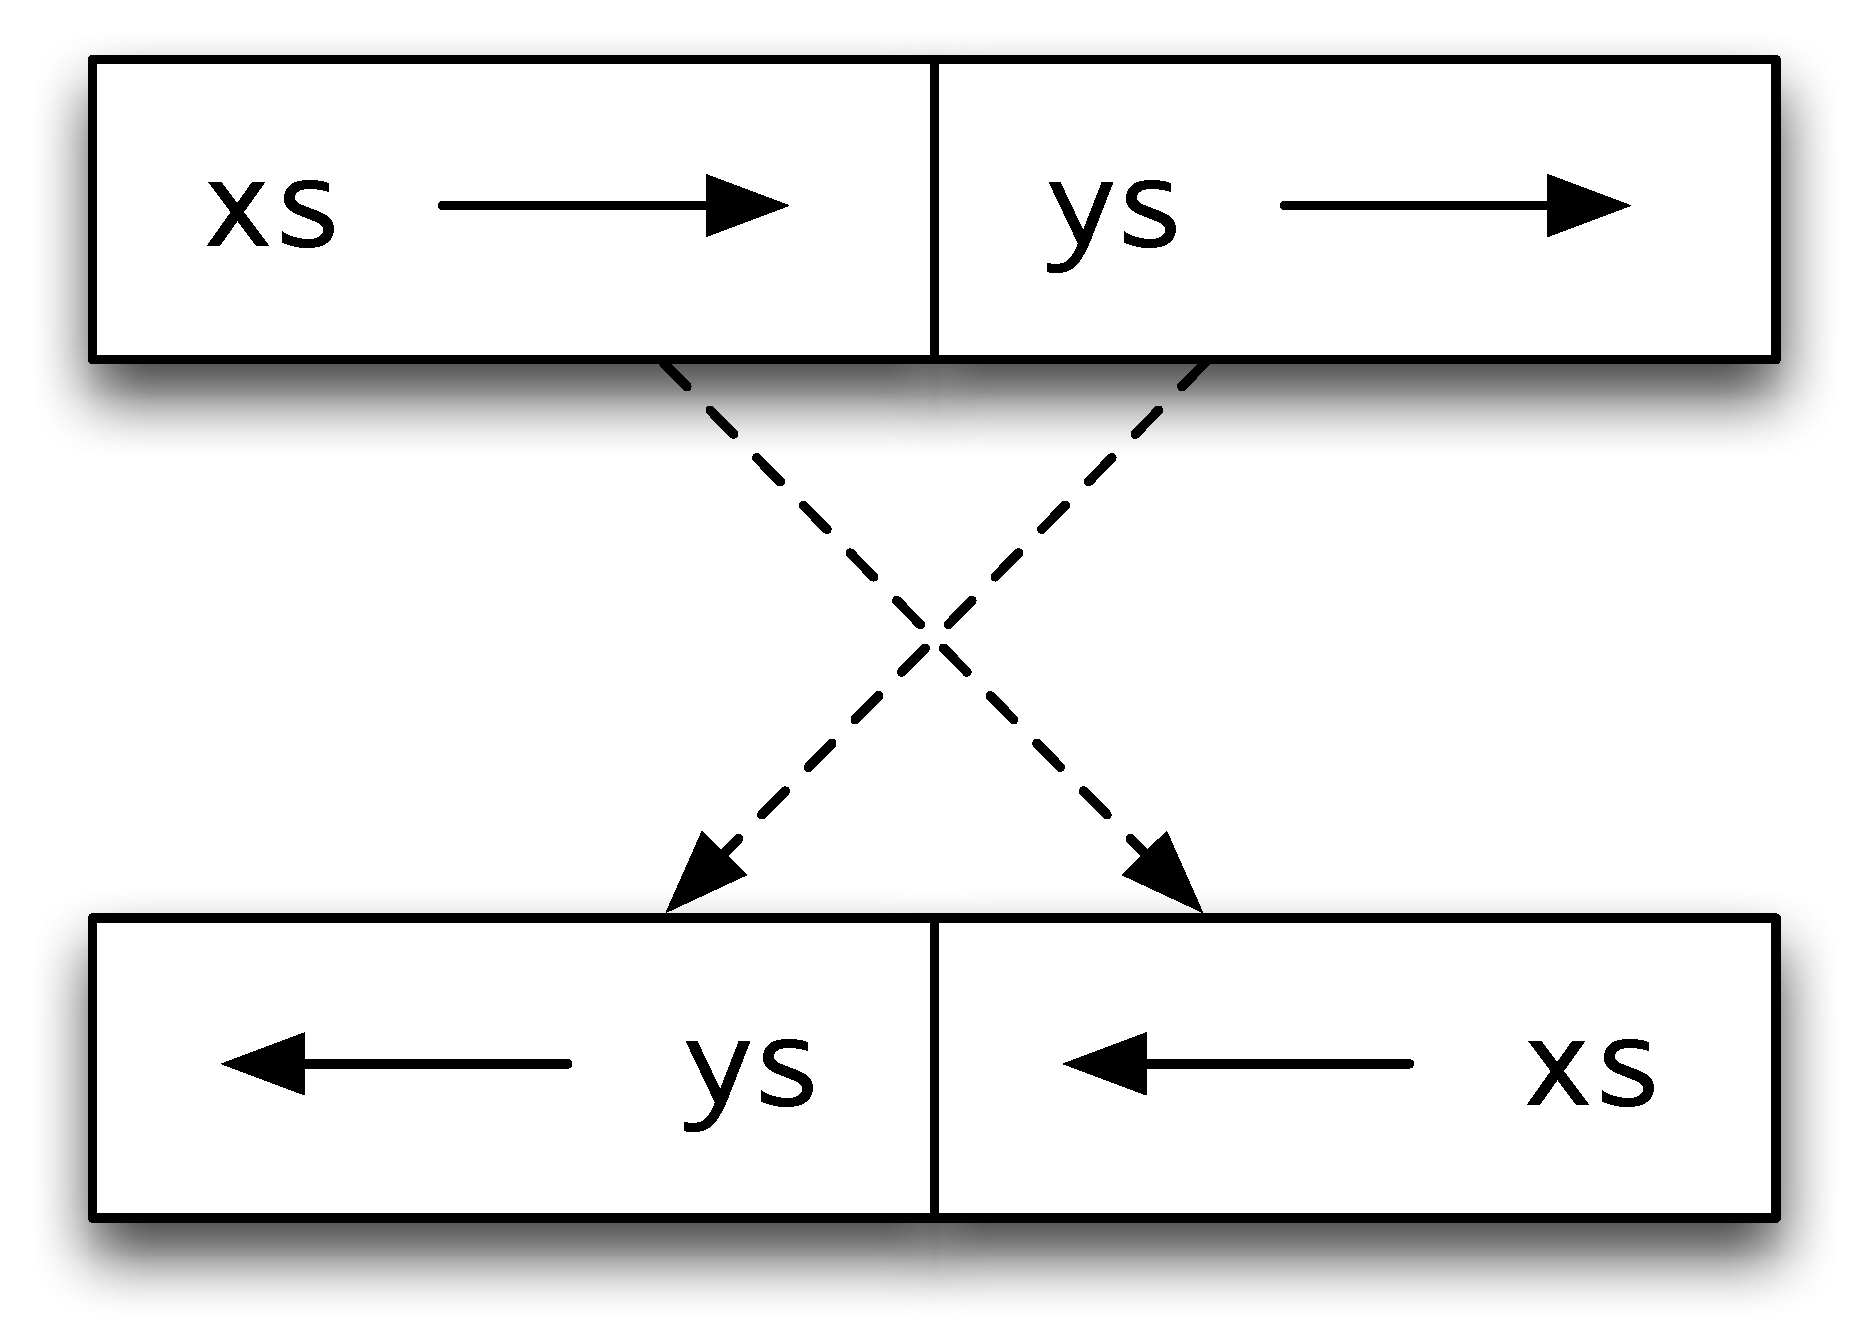
\includegraphics[width=2.5in]{Pictures/reverseSwap.pdf}
\end{center}
\caption{Reversing the list \texttt{xs++ys}}
\label{reverseSwap}
\end{figure}


\subsubexample*{2. \texttt{reverse} and \texttt{++}}\minx{reverse}\minx{++}

What happens when we reverse the join of two lists, \texttt{xs++ys}? The process is illustrated in Figure{reverseSwap}.
Each list is reversed, and they are swapped. In formal terms, 
\begin{alltt}
reverse (xs ++ ys) = reverse ys ++ reverse xs\hfill(reverse++)
\end{alltt}
where we define
\begin{alltt}
reverse []     = []\hfill(reverse.1)
reverse (z:zs) = reverse zs ++ [z]\hfill(reverse.2)
\end{alltt}
We will try to prove \texttt{(reverse++)} for all finite lists
\texttt{xs} and \texttt{ys}
by induction over \texttt{xs}.

\subparagraph*{Statement} The base case is
\begin{alltt}
reverse ([] ++ ys) = reverse ys ++ reverse []\hfill(base)
\end{alltt} 
and the induction goal is 
\begin{alltt}
reverse ((x:xs) ++ ys) = reverse ys ++ reverse (x:xs)\hfill(ind)
\end{alltt}
which is to be proved using the assumption
\begin{alltt}
reverse (xs ++ ys) = reverse ys ++ reverse xs\hfill(hyp)
\end{alltt}

\subparagraph*{Base} Simplifying both sides of \texttt{(base)} gives us 
\begin{alltt}
reverse ([] ++ ys) 
  = reverse ys \hfill \textrm{by }(++.1)

reverse ys ++ reverse []
  = reverse ys ++ [] \hfill \textrm{by }(reverse.1)
\end{alltt}
but we can prove the two equal only if we can show that appending an empty
list to the end of a list is an \textbf{identity} operation, that
is\index{identity}
\begin{alltt}
xs ++ [] = xs\hfill(++.3)
\end{alltt}
We leave a proof of this by induction over \texttt{xs} as an exercise for the reader.

\subparagraph*{Induction} Again, we look at the two sides of the equation, left-hand
side first.
\begin{alltt}
reverse ((x:xs) ++ ys) 
  = reverse (x:(xs ++ ys)) \hfill \textrm{by }(++.2)
  = reverse (xs ++ ys) ++ [x]  \hfill \textrm{by }(reverse.2)
  = (reverse ys ++ reverse xs) ++ [x]  \hfill \textrm{by }(hyp)
\end{alltt}
Examining the right-hand side, we have
\begin{alltt}
reverse ys ++ reverse (x:xs)
  = reverse ys ++ (reverse xs ++ [x]) \hfill \textrm{by }(reverse.2)
\end{alltt}
Now, these two are {\em almost\/} equal, except that the joins are
bracketed differently. We need another general property of \texttt{++},
namely that it is \textbf{associative}:
\begin{alltt}
xs ++ (ys ++ zs) = (xs ++ ys) ++ zs\hfill(++.4)
\end{alltt}
the proof of which we again leave as an exercise.\blackbox
\end{example}

\noindent This proof is instructive: it shows that often in proofs we use other
theorems or lemmas (the mathematician's term for a `little theorem') on
the way. If we do any serious proof we will build up a library of these
lemmas, with \texttt{(++.3)} and \texttt{(++.4)} being basic results about
\texttt{++} which we will call upon almost without thinking. We would expect
this library to resemble the standard prelude: it would contain all those
theorems which link the prelude functions and which will be called into use
whenever we use prelude functions. Many of the exercises at the end of the
section ask you to prove theorems concerning prelude functions.

\begin{figure}[t]\index{QuickCheck!properties over \texttt{[a]}}
\beware{QuickCheck and properties over \texttt{[a]}}{
If we test the QuickCheck property
\begin{alltt}
prop\_reversePlusPlus :: Eq a => [a] -> [a] -> Bool\\
\ \\
prop\_reversePlusPlus xs ys =\\
\hspace*{0.8cm}reverse (xs ++ ys) == reverse ys ++ reverse xs
\end{alltt}
we find that it holds. Fine, but if we check this property:
\begin{alltt}
prop\_reversePlusPlusOops :: Eq a => [a] -> [a] -> Bool\\
\ \\
prop\_reversePlusPlusOops xs ys =\\
\hspace*{0.8cm}reverse (xs ++ ys) == reverse xs ++ reverse ys
\end{alltt}
we find that this holds too! 

\medskip
What is happening here? The problem is that when we check a generic property -- that is one over a polymorphic type -- then it is in fact checked over a default type. This default type is \texttt{()}, which has exactly one element, also \texttt{()}. The incorrect property \emph{is} correct over lists of that type, because all their elements are the same!

\medskip
In order to restore sanity, it is enough to change the properties to a suitable non-generic type, using a type declaration like this:
\begin{alltt}
prop\_reversePlusPlusOops :: [Integer] -> [Integer] -> Bool
\end{alltt}
}
\end{figure}


\begin{exercises}

\item
Prove the properties for functions over \texttt{Picture} first discussed in Section \ref{proof}, that is, for all finite \texttt{pic}:
\begin{alltt}
flipV (flipH pic) = flipH (flipV pic)
flipV (flipV pic) = pic
flipH (flipV pic) = pic
\end{alltt}


\item
Look again at the properties for functions over \texttt{Picture} discussed in Section \ref{picturesAgain}, and prove those properties which should hold for all pictures.




\item
Prove for all finite \texttt{xs} and \texttt{ys} that
\begin{alltt}
sum (xs ++ ys) = sum xs + sum ys	\hfill(sum++)
\end{alltt}

\item
Prove the two rules for \texttt{++}:
\begin{alltt}
xs ++ [] = xs\hfill(++.3)
xs ++ (ys ++ zs) = (xs ++ ys) ++ zs\hfill(++.4)
\end{alltt}
for all finite \texttt{xs}, \texttt{ys} and \texttt{zs}.

\item
Show for all finite \texttt{xs} that
\begin{alltt}
sum (reverse xs)    = sum xs
length (reverse xs) = length xs
\end{alltt}
What common factors can you see in your two proofs?

\item
Show for all finite integer lists \texttt{xs} and \texttt{ys} that
\begin{alltt}
elem z (xs ++ ys) = elem z xs || elem z ys
\end{alltt}

\item
Show for all finite lists \texttt{ps} that
\begin{alltt}
zip (fst (unzip ps)) (snd (unzip ps)) = ps
\end{alltt}
Under what conditions on \texttt{xs} and \texttt{ys} is it the case that
\begin{alltt}
unzip (zip xs ys) = (xs,ys)
\end{alltt}
when \texttt{unzip} is defined by
\begin{alltt}\minx{unzip}
unzip [] = ([],[])
unzip ((x,y):ps) 
  = (x:xs,y:ys)
    where
    (xs,ys) = unzip ps                   
\end{alltt}
Give a proof in that case.

\item
\mbox{[Harder]} Show for all finite \texttt{xs} and defined \texttt{n} that
\begin{alltt}
take n xs ++ drop n xs = xs
\end{alltt}


\item
Write QuickCheck properties for the propositions that you have proved, and check that they indeed hold.

\end{exercises}
\index{induction|)}


\section{Generalizing the proof goal}
\label{genPrf}
\index{induction!generalizing the goal}

It is not always easy to build a proof in a straightforward way, by induction
over a goal we set ourselves. In this section we explore an example in which
we are able to build a proof of the property we
seek only after two false starts. 
The section is more challenging than the rest of the chapter and can safely
be omitted on first reading.


\subsection*{The shunting function}

The \texttt{shunt} function moves the elements from one list onto another, like this
\begin{alltt}
shunt :: [a] -> [a] -> [a]\minx{shunt}
\bl
shunt []     ys = ys\hfill (shunt.1)
shunt (x:xs) ys = shunt xs (x:ys) \hfill (shunt.2)
\end{alltt}
Starting with an empty second argument, we have
\begin{alltt}
shunt [2,3,1] []
\step shunt [3,1] [2]
\step shunt [1] [3,2]
\step shunt [] [1,3,2]
\step [1,3,2]
\end{alltt}
and so we can reverse lists using this function:
\begin{alltt}
rev :: [a] -> [a]\minx{rev}
rev xs = shunt xs []\hfill (rev.1)
\end{alltt}
Now we turn to looking at properties of the \texttt{rev} function.

\subsection*{First proof attempt}

Reversing a list twice should give us back the list we started with, and so
we aim to prove that 
\begin{alltt}
rev (rev xs) = xs \hfill Q(xs)
\end{alltt}
for
all finite lists \texttt{xs}. The base case is easily established, but when we
look at the induction step, we meet our first problem:
\begin{alltt}
rev (rev (x:xs))
  = shunt (shunt (x:xs) []) [] \hfill {\rm by} (rev.1)
  = shunt (shunt xs [x]) []\hfill {\rm by} (shunt.2)
\end{alltt} 
This has no direct relationship to the induction
hypothesis, which mentions only the function \texttt{rev}. A clue to the problem
is that \texttt{rev} is not the function defined by recursion --- it is simply a
specialization of \texttt{shunt}. Can we find a {\em generalization\/} of 
\texttt{Q(xs)} which talks explicitly about \texttt{shunt} and which is to be proved by
induction? 

In general the effect of \texttt{shunt xs ys} is to give
\begin{alltt}
(reverse xs) ++ ys
\end{alltt}
If we reverse this list, we should get
\begin{alltt}
(reverse ys) ++ xs
\end{alltt}
(try some examples!) and so we should be able to prove that
\begin{alltt}
shunt (shunt xs ys) [] = shunt ys xs
\end{alltt}
When \texttt{ys} is replaced by 
\texttt{[]}, we get \texttt{Q(xs)}. We therefore aim to prove this generalization.

\subsection*{Second proof attempt}

Our aim is to show
\begin{alltt}
shunt (shunt xs ys) [] = shunt ys xs
\end{alltt}
for all finite lists \texttt{xs} and \texttt{ys}. In the case that \texttt{xs} is {\mi
[]}, the proof is simple. Now we look at the induction step:
\begin{alltt}
shunt (shunt (x:xs) ys) [] 
  = shunt (shunt xs (x:ys)) [] \hfill {\rm by} (shunt.2)
\end{alltt}
We would now like to claim by induction that this is equal to \texttt{shunt
(x:ys) xs}, but to do this we need the induction hypothesis to give the result
that
\begin{alltt}
shunt (shunt xs (x:ys)) [] = shunt (x:ys) xs
\end{alltt}
rather than 
\begin{alltt}
shunt (shunt xs ys) [] = shunt ys xs\end{alltt}
To get around this, we strengthen the induction hypothesis to become
\begin{alltt}
shunt (shunt xs zs) [] = shunt zs xs {\rm for all finite lists} zs\end{alltt}
so that in particular it will hold when \texttt{(x:ys)} replaces \texttt{zs}. We now
try again.

\subsection*{The successful proof attempt} 

In logical notation, our goal is to prove
\begin{alltt}
\all{}zs (shunt (shunt xs zs) [] = shunt zs xs)
\end{alltt}
\index{\forall@$\forall$}
for all finite \texttt{xs} by induction.

\subparagraph*{Statement} Now we can state what is required. The base case is
\begin{alltt}
\all{}zs (shunt (shunt [] zs) [] = shunt zs []) \hfill (base)
\end{alltt}
and the induction step is to prove
\begin{alltt}
\all{}zs (shunt (shunt (x:xs) zs) [] = shunt zs (x:xs)) \hfill (ind)
\end{alltt}
assuming the induction hypothesis
\begin{alltt}
\all{}zs (shunt (shunt xs zs) [] = shunt zs xs) \hfill (hyp)
\end{alltt}

\subparagraph*{Base} In the base case we prove 
\begin{alltt}
\all{}zs (shunt (shunt [] zs) [] = shunt zs []) \hfill (base)
\end{alltt}
by proving it for an arbitrary \texttt{zs}. 
The left-hand side simplifies 
to the right-hand side in one step.
\begin{alltt}
shunt (shunt [] zs) []
  = shunt zs [] \hfill {\rm by} (shunt.1)
\end{alltt}

\subparagraph*{Induction} 
As in the base case, we prove  
\begin{alltt}
\all{}zs (shunt (shunt (x:xs) zs) [] = shunt zs (x:xs)) \hfill (ind)
\end{alltt}
by proving it for an arbitrary \texttt{zs}. Simplifying the left-hand side, we
have
\begin{alltt}
shunt (shunt (x:xs) zs) [] 
  = shunt (shunt xs (x:zs)) [] \hfill {\rm by} (shunt.2)
\end{alltt}
Now, by \texttt{(hyp)}, where we take the particular value \texttt{(x:zs)} to replace the
universally quantified variable \texttt{zs},
\begin{alltt}
  = shunt (x:zs) xs \hfill {\rm by} (hyp)
  = shunt zs (x:xs) \hfill {\rm by} (shunt.2)
\end{alltt}
This is the right-hand side, and so the proof is complete for an arbitrary
\texttt{ys}, giving a proof of \texttt{(ind)}, and completing the induction proof.
\blackbox

\medskip
\noindent
This example shows that we may have to generalize what has to be proved in
order for induction proofs to work. This seems paradoxical: we are making it
harder for ourselves, apparently. We are in one way, but at the same time we
make the induction hypothesis {\em stronger}, so that we have {\em more\/}
resources to use when proving the induction step.


\begin{exercises}
\item
Prove for all finite lists \texttt{xs} and \texttt{ys} that
\begin{alltt}
rev (xs ++ ys) = rev ys ++ rev xs
\end{alltt}

\item
Using the function
\begin{alltt}
facAux :: Integer -> Integer -> Integer
facAux 0 p = p
facAux n p = facAux (n-1) (n*p)
\end{alltt}
we can define
\begin{alltt}
fac2 n = facAux n 1
\end{alltt}
Prove that for all defined natural numbers \texttt{n},
\begin{alltt}
fac n = fac2 n
\end{alltt}


\item
Write a property expressing that the old and new \texttt{reverse} functions have the same behaviour.

\item
Write a property expressing that the old and new factorial functions have the same behaviour. What happens to the QuickCheck of the property if you allow arbitrary integer inputs to the factorial functions? how can you remedy this?




\end{exercises}


\begin{summary}
This chapter has shown that we can give Haskell programs a logical reading
which allows us to reason about them. Central to reasoning
about lists is the principle of structural induction, which does
for proof what primitive recursion does for definitions.

We gave a collection of hints about how we can build
proofs for functional programs, and illustrated these by giving a number of results
for common prelude functions such as \texttt{sum}, \texttt{++} and
\texttt{length}, as well as exercises involving others. We also saw how QuickCheck could be used to check whether or not a property appears to hold: this is a very useful way of making a `sanity check' of a property before we try to prove it.


\index{proof|)}

\end{summary}
%\end{document}
